\documentclass{article}
\usepackage[utf8]{inputenc}
\usepackage{graphicx}
\usepackage{float}
\begin{document}


\begin{titlepage}
\begin{center}
{\Huge Documentation of Computational Intelligence and Deep Learning project \par}
\vspace{18mm}
{\huge Marco Parola \par}
{\huge Stefano Poleggi \par}
\vspace{18mm}
A.Y. 2020-2021
\end{center}

\end{titlepage}

% ----- INDICE -----
\tableofcontents\thispagestyle{empty}
\clearpage


% --------------------------------------- INTRO -------------------------------------------------------
\section{Introduction}
\subsection{Data distribution}
The dataset of this project has been created from the well known dataset CBIS DDSM (Curated Breast Imaging Subset of Digital Database for Screening Mammography), considering a sub number of radiography already labeled on the following classes:
\begin{itemize}
\item 1 Mass, Benign 
\item 2 Mass, Malignant
\item 3 Calcification, Benign
\item 4 Calcification, Malignant
\end{itemize}
Moreover for each image belongs to the previous classes is present another image extracted from the same radiography, but representing a healthy portion.\\
The following plot show the number of sample for each class belongs to the trainingset.\\
\begin{minipage}{\linewidth}
\begin{center}
\vspace{3mm}
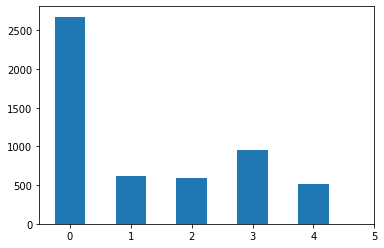
\includegraphics[scale=0.6]{./img/distribution1.png} 
\vspace{3mm}
\end{center}
\end{minipage}
The following plot show the number of sample for each class belongs to the testset.\\
\begin{minipage}{\linewidth}
\begin{center}
\vspace{3mm}
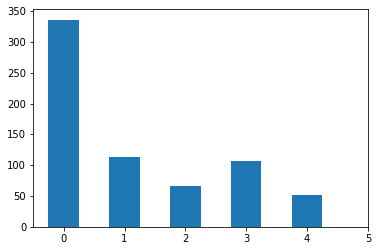
\includegraphics[scale=0.6]{./img/distribution2.png} 
\vspace{3mm}
\end{center}
\end{minipage}
The following plot show the number of sample belonging to the class Mass and to the class Calcification.\\
\begin{minipage}{\linewidth}
\begin{center}
\vspace{3mm}
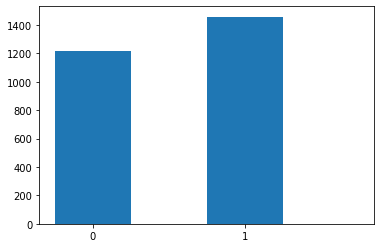
\includegraphics[scale=0.6]{./img/distribution3.png} 
\vspace{3mm}
\end{center}
\end{minipage}
The following plot show the number of sample belonging to the class Benign and to the class Malignant.\\
\begin{minipage}{\linewidth}
\begin{center}
\vspace{3mm}
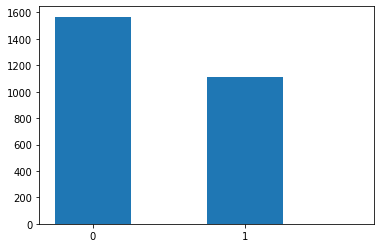
\includegraphics[scale=0.6]{./img/distribution4.png} 
\vspace{3mm}
\end{center}
\end{minipage}

\subsection{Benign-Malignant classification VS Mass-Calcification classification}
During all the experiments we observed a substantial difference between the classification benign-malignant and the classification mass-calcification.\\ 
In our opinion this could be caused by a strong similarity between mass benign and mass malignant (same for calcification) with respect to benign mass and benign calcification (same for malignant).

\subsection{Compute shuffle on the dataset}
During the first experiments we observed some picks on the accuracy and loss plots, we solved this problem simply preprocessing the data, computing a shuffle phase, in which we computed a parmutation on the images and the same transofmation on the labels, in order to maintain the consistency.

\begin{verbatim}
training = []
for i in range(len(trainingSet)):
  training.append((trainingSet[i], trainingLabels[i]))

training = np.array(training)
np.random.shuffle(training)

\end{verbatim}


\clearpage
% --------------------------------------- TASK 1 -------------------------------------------------------
\section{Task 1}
We read the following paper to study the approcches followed by some researches:
\begin{itemize}
\item Transfer Learning with Convolutional Neural Network for Early Gastric Cancer Classification on Magnifiying Narrow-Band Imaging Images, published in 2018 25th IEEE International Conference on Image Processing (ICIP).
\item Multi-View Feature Fusion Based Four ViewsModel for Mammogram Classification UsingConvolutional Neural Network,published in 2019 26th November IEEE.
\item Analysis on the Dropout Effect in Convolutional Neural Networks
\end{itemize}
Starting from these papers, we took ispiration in different aspects.

\subsection{Pretrained Convolutional Neural Networks}
Considering different experiments described on the journals, we detected some pretrained CNN most used for medical images classification:
\begin{itemize}
\item AlexNet
\item VGG16
\item GoogLeNet
\item ResNet
\end{itemize}
We analyzed this topics more in detail on section related to the task 3.\\

\subsection{Setting of Hyper-parameters}
We took inspiration to set the hyper-parameters with wich we started training our models from the second and third journal.\\
In our experiments we used the same learning rate values, the activation functions and the number of convolutional layers (in the 'from Scratch' tasks), used in \textbf{Multi-View Feature Fusion Based Four ViewsModel for Mammogram Classification UsingConvolutional Neural Network} paper.\\
Moreover from this paper we took the hyper-parameters of the \textit{ImageDataGenerator}, thanks wich we computed the data augmentation:
\begin{itemize}
\item Rotation = 90
\item Horizontal shift range = 0.2
\item Vertical shift range = 0.2
\item Zoom range = 0.2
\item Shear = 20
\item Fill model = 'nearest' \\
\end{itemize}
On section related to the task 2.2 we will show the hyperparameters that we set, starting from these.\\
From the \textbf{Analysis on the Dropout Effect in Convolutional Neural Networks} journal we took inspiration about the dropout rate values, in particular we used the following guidelines:
\begin{itemize}
\item for dropout rate between convolutional layers we used a value between 0.1 and 0.2 
\item for dropout rate between dense layers we used a haigher value: 0.5\\
\end{itemize}



\clearpage
% --------------------------------------- TASK 2 -------------------------------------------------------
\section{Task 2}
Task 2 consists in building from scratch different convolotional neural networks able to compute the following classification:
\begin{itemize}
\item Mass - Calcification
\item Benign - Malignant
\end{itemize}
We have carried out this task adopting an approach "trial and error", in this way we found a our best classifier step by step.

% --------------------------------------- TASK 2.1 -------------------------------------------------------
\subsection{Task 2.1, Mass - Calcification}
We compiled our deep nural networks using two optimizers:
\begin{itemize}
\item adam
\item RMSprop
\end{itemize}
In all these experiments we used an early stopping condition, we set the \textit{patience} value euristicly equal to 10. \\
Moreover exploiting the \textit{restore\_best\_weights} itroduced in keras 2.2.3 we set the best weights of the model found previously.
\subsubsection{Model 1}

\begin{itemize}
\item Optimizer: Adam, learning rate = 0.001 (default)
\item Early stopping condition: monitoring loss on validation set, patience = 10
\item Dense hidden layers: 2
\item Activation function: softmax
\end{itemize}

\begin{verbatim}


              precision    recall  f1-score   support

           0       0.80      0.81      0.81       179
           1       0.78      0.77      0.78       157

    accuracy                           0.79       336
   macro avg       0.79      0.79      0.79       336
weighted avg       0.79      0.79      0.79       336


0s 17ms/step - loss: 0.4683 - accuracy: 0.7887

\end{verbatim}



\begin{figure}[h]
    \centering
    \begin{minipage}{0.45\textwidth}
        \centering
        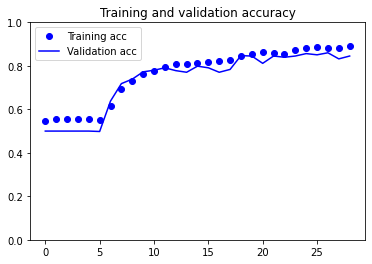
\includegraphics[scale=0.46]{./img/scratchVal1.png}
    \end{minipage}\hfill
    \begin{minipage}{0.45\textwidth}
        \centering
        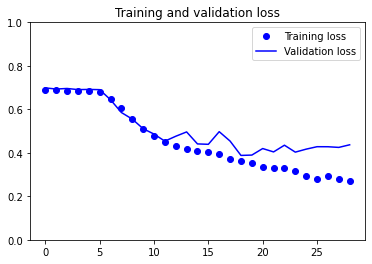
\includegraphics[scale=0.46]{./img/scratchLoss1.png}
    \end{minipage}
\end{figure}

\begin{center}
\begin{minipage}{0.45\textwidth}
        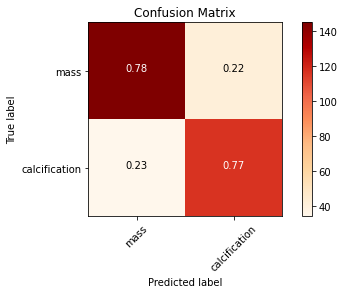
\includegraphics[scale=0.6]{./img/cmScratch1.png}
    \end{minipage}
\end{center}

% ---------
\subsubsection{Model 2}
We modified the architecture of the network, adding one more convolutional layer before the first two max-pooling layers.

\begin{itemize}
\item Optimizer: RMSProp, learning rate = 1e-4
\item Early stopping condition: monitoring loss on validation set, patience = 10
\item Dense hidden layers: 1
\item Activation function: sigmoid
\end{itemize}

\begin {verbatim}


              precision    recall  f1-score   support

           0       0.84      0.88      0.86       179
           1       0.86      0.82      0.84       157

    accuracy                           0.85       336
   macro avg       0.85      0.85      0.85       336
weighted avg       0.85      0.85      0.85       336

1s 44ms/step - loss: 0.3996 - accuracy: 0.8512

\end{verbatim}

\begin{figure}[h]
    \centering
    \begin{minipage}{0.45\textwidth}
        \centering
        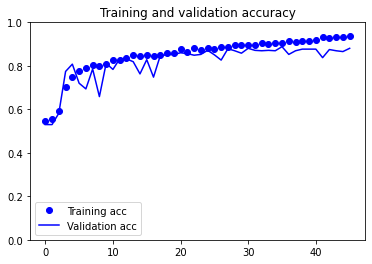
\includegraphics[scale=0.46]{./img/scratchVal2.png}
    \end{minipage}\hfill
    \begin{minipage}{0.45\textwidth}
        \centering
        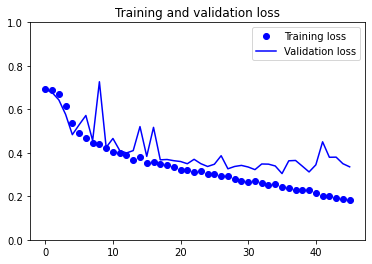
\includegraphics[scale=0.46]{./img/scratchLoss2.png}
    \end{minipage}
\end{figure}

\begin{center}
\begin{minipage}{0.45\textwidth}
        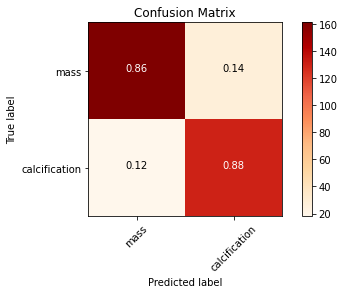
\includegraphics[scale=0.6]{./img/cmScratch2.png}
    \end{minipage}
\end{center}
By applying this modification to the previous neural network, we can observe an improvement on the accuracy value of about 9\% and a decrease on the loss of about 18\%.


% ---------
\subsubsection{DropOut Model}
In the previous loss function plot we can observe a slight deviation between the loss function of the training set and validation set, that could imply our model is affected by overfitting. In order to solve this problem we introduce some dropout layers has seen in "Analysis on the Dropout Effect in Convolutional Neural Networks" journal, with a percentage equal to 0,15.

\begin{itemize}
\item Optimizer: RMSProp, learning rate = 1e-4
\item Early stopping condition: monitoring loss on validation set, patience = 10
\item Dense hidden layers: 1
\item Activation function: sigmoid
\end{itemize}

\begin {verbatim}

Model: "sequential_6"
_________________________________________________________________
Layer (type)                 Output Shape              Param #   
=================================================================
conv2d_35 (Conv2D)           (None, 150, 150, 32)      320       
_________________________________________________________________
conv2d_36 (Conv2D)           (None, 150, 150, 64)      18496     
_________________________________________________________________
dropout_4 (Dropout)          (None, 150, 150, 64)      0         
_________________________________________________________________
max_pooling2d_25 (MaxPooling (None, 75, 75, 64)        0         
_________________________________________________________________
conv2d_37 (Conv2D)           (None, 75, 75, 64)        36928     
_________________________________________________________________
conv2d_38 (Conv2D)           (None, 75, 75, 64)        36928     
_________________________________________________________________
dropout_5 (Dropout)          (None, 75, 75, 64)        0         
_________________________________________________________________
max_pooling2d_26 (MaxPooling (None, 37, 37, 64)        0         
_________________________________________________________________
conv2d_39 (Conv2D)           (None, 37, 37, 128)       73856     
_________________________________________________________________
dropout_6 (Dropout)          (None, 37, 37, 128)       0         
_________________________________________________________________
max_pooling2d_27 (MaxPooling (None, 18, 18, 128)       0         
_________________________________________________________________
conv2d_40 (Conv2D)           (None, 18, 18, 256)       295168    
_________________________________________________________________
dropout_7 (Dropout)          (None, 18, 18, 256)       0         
_________________________________________________________________
max_pooling2d_28 (MaxPooling (None, 9, 9, 256)         0         
_________________________________________________________________
flatten_6 (Flatten)          (None, 20736)             0         
_________________________________________________________________
dense_14 (Dense)             (None, 256)               5308672   
_________________________________________________________________
dense_15 (Dense)             (None, 2)                 514       
=================================================================
Total params: 5,770,882
Trainable params: 5,770,882
Non-trainable params: 0
_________________________________________________________________




              precision    recall  f1-score   support

           0       0.81      0.91      0.85       179
           1       0.87      0.75      0.81       157

    accuracy                           0.83       336
   macro avg       0.84      0.83      0.83       336
weighted avg       0.84      0.83      0.83       336

1s 44ms/step - loss: 0.3807 - accuracy: 0.8333

\end{verbatim}

\begin{figure}[h]
    \centering
    \begin{minipage}{0.45\textwidth}
        \centering
        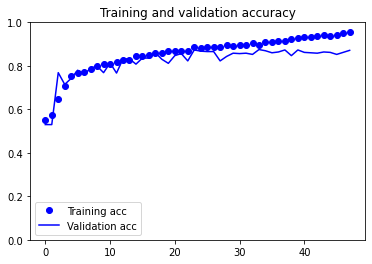
\includegraphics[scale=0.46]{./img/scratchValDrop.png}
    \end{minipage}\hfill
    \begin{minipage}{0.45\textwidth}
        \centering
        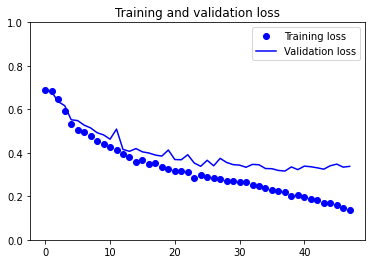
\includegraphics[scale=0.46]{./img/scratchLossDrop.png}
    \end{minipage}
\end{figure}

\begin{center}
\begin{minipage}{0.45\textwidth}
        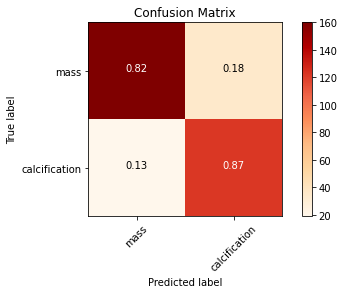
\includegraphics[scale=0.6]{./img/cmScratchDrop.png}
    \end{minipage}
\end{center}
There is a bit decrese both on the loss and accurancy, by looking at the plot of loss value we can observe the validation curve is more regular than the previous experiments, solving partially the overfitting problem.

% ---------
\subsubsection{Model 4}
We also try to improve the performance of our model, modifying the dense layers of the nettwork and adding one more hidden layer.
\begin{itemize}
\item Optimizer: RMSProp, learning rate = 1e-4
\item Early stopping condition: monitoring loss on validation set, patience = 10
\item Dense hidden layers: 2
\item Activation function: sigmoid
\end{itemize}

\begin {verbatim}

              precision    recall  f1-score   support

           0       0.80      0.92      0.86       179
           1       0.89      0.74      0.81       157

    accuracy                           0.84       336
   macro avg       0.85      0.83      0.83       336
weighted avg       0.84      0.84      0.83       336

1s 44ms/step - loss: 0.3909 - accuracy: 0.8363

\end{verbatim}

\begin{figure}[h]
    \centering
    \begin{minipage}{0.45\textwidth}
        \centering
        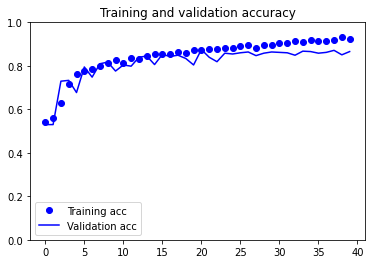
\includegraphics[scale=0.46]{./img/scratchVal4.png}
    \end{minipage}\hfill
    \begin{minipage}{0.45\textwidth}
        \centering
        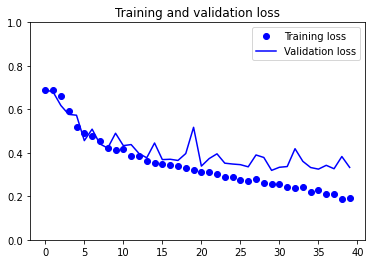
\includegraphics[scale=0.46]{./img/scratchLoss4.png}
    \end{minipage}
\end{figure}

\begin{center}
\begin{minipage}{0.45\textwidth}
        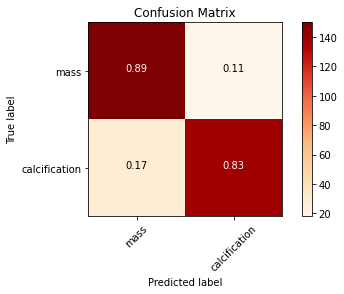
\includegraphics[scale=0.6]{./img/cmScratch4.png}
    \end{minipage}
\end{center}
We couldn't see any improvements both on loss and accuracy, so we can conclude that the added layer is not usefull.


% ---------
\subsubsection{Model 5}
In the last trial we change the activation function of the last layer from \textit{sigmoid} to \textit{softmax}, but also this change brought no improvement.

\begin{itemize}
\item Optimizer: RMSProp, learning rate = 1e-4
\item Early stopping condition: monitoring loss on validation set, patience = 10
\item Dense hidden layers: 1
\item Activation function: softmax
\end{itemize}

\begin {verbatim}


              precision    recall  f1-score   support

           0       0.81      0.89      0.85       179
           1       0.86      0.76      0.81       157

    accuracy                           0.83       336
   macro avg       0.84      0.83      0.83       336
weighted avg       0.84      0.83      0.83       336

0s 44ms/step - loss: 0.4027 - accuracy: 0.8333

\end{verbatim}

\begin{figure}[h]
    \centering
    \begin{minipage}{0.45\textwidth}
        \centering
        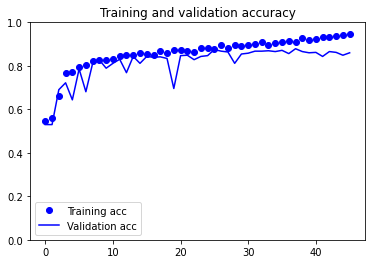
\includegraphics[scale=0.46]{./img/scratchVal5.png}
    \end{minipage}\hfill
    \begin{minipage}{0.45\textwidth}
        \centering
        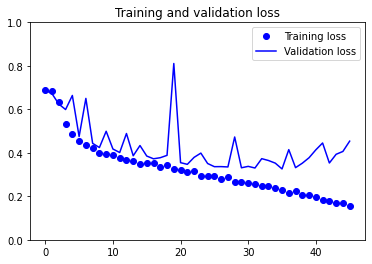
\includegraphics[scale=0.46]{./img/scratchLoss5.png}
    \end{minipage}
\end{figure}

\begin{center}
\begin{minipage}{0.45\textwidth}
        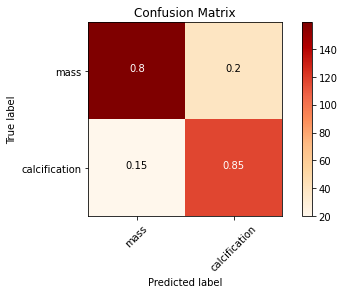
\includegraphics[scale=0.6]{./img/cmScratch5.png}
    \end{minipage}
\end{center}

% ------
\subsection{Conclusion task 2.1}
We ploted the roc curve related to each of the built models and we compared them.
\begin{center}
\begin{minipage}{0.45\textwidth}
        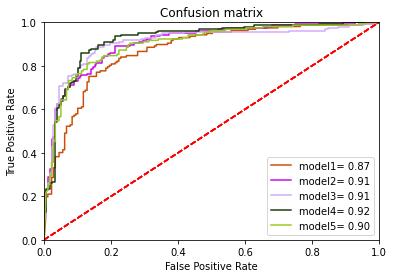
\includegraphics[scale=0.6]{./img/rocScratch.png}
    \end{minipage}
\end{center}


\clearpage
% --------------------------------------- TASK 2.2 -------------------------------------------------------
\subsection{Task 2.2, Benign - Malignant}
Also in this case we set an early stopping condition, reusing the same hyperparameters.

\subsubsection{Model 1}
In the first trial of benign-malignant classification we built a different model, composed by less layers.

\begin{itemize}
\item Optimizer: RMSProp, learning rate = 1e-4
\item Early stopping condition: monitoring loss on validation set, patience = 10
\item Dense hidden layers: 1
\item Dropout layer: rate = 0.5
\item Activation function: softmax
\end{itemize}

\begin{verbatim}

Model: "sequential_4"
_________________________________________________________________
Layer (type)                 Output Shape              Param #   
=================================================================
conv2d_16 (Conv2D)           (None, 150, 150, 32)      320       
_________________________________________________________________
max_pooling2d_16 (MaxPooling (None, 75, 75, 32)        0         
_________________________________________________________________
conv2d_17 (Conv2D)           (None, 75, 75, 64)        18496     
_________________________________________________________________
max_pooling2d_17 (MaxPooling (None, 37, 37, 64)        0         
_________________________________________________________________
conv2d_18 (Conv2D)           (None, 37, 37, 64)        36928     
_________________________________________________________________
max_pooling2d_18 (MaxPooling (None, 18, 18, 64)        0         
_________________________________________________________________
conv2d_19 (Conv2D)           (None, 18, 18, 128)       73856     
_________________________________________________________________
max_pooling2d_19 (MaxPooling (None, 9, 9, 128)         0         
_________________________________________________________________
flatten_4 (Flatten)          (None, 10368)             0         
_________________________________________________________________
dense_8 (Dense)              (None, 256)               2654464   
_________________________________________________________________
dropout_4 (Dropout)          (None, 256)               0         
_________________________________________________________________
dense_9 (Dense)              (None, 2)                 514       
=================================================================
Total params: 2,784,578
Trainable params: 2,784,578
Non-trainable params: 0
_________________________________________________________________



              precision    recall  f1-score   support

           0       0.76      0.68      0.71       219
           1       0.50      0.60      0.54       117

    accuracy                           0.65       336
   macro avg       0.63      0.64      0.63       336
weighted avg       0.67      0.65      0.65       336

0s 9ms/step - loss: 0.6349 - accuracy: 0.6488

\end{verbatim}



\begin{figure}[h]
    \centering
    \begin{minipage}{0.45\textwidth}
        \centering
        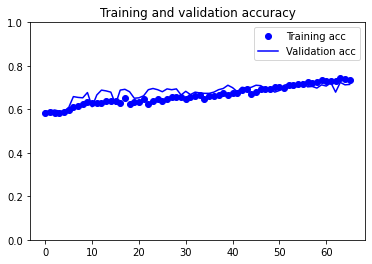
\includegraphics[scale=0.46]{./img/scratchVal1_2.png}
    \end{minipage}\hfill
    \begin{minipage}{0.45\textwidth}
        \centering
        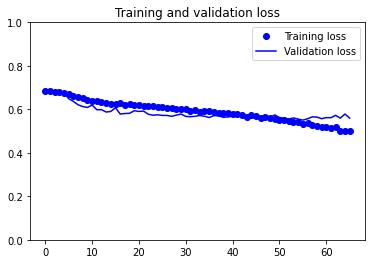
\includegraphics[scale=0.46]{./img/scratchLoss1_2.png}
    \end{minipage}
\end{figure}

\begin{center}
\begin{minipage}{0.45\textwidth}
        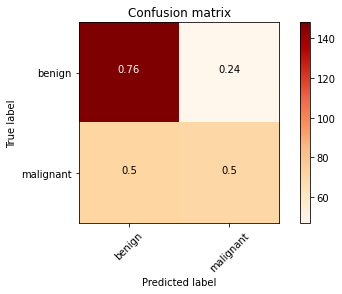
\includegraphics[scale=0.6]{./img/cmScratch1_2.png}
    \end{minipage}
\end{center}

\subsubsection{Deal with unbalanced dataset, using data augmentation}
From the confusion matrix of the first trial we can observe the major part of the wrong classification has been computed on the class 'Malignant'. This could be a problem, considering that these cases are more important to detect.\\
In order to try to solve this unbalanced classification, we compute a data augmentation task, using \textit{ImageDataGenerator} object of keras.preprocessing package.

\begin{verbatim}

dataGenerator = ImageDataGenerator(
      rotation_range=45,
      width_shift_range=0.15,
      height_shift_range=0.15,
      shear_range=20,
      zoom_range=0.15,
      horizontal_flip=True,
      fill_mode='reflect')

\end{verbatim}
To set the parameters of ImageDataGenerator, we took inspiration from "Multi-View Feature Fusion Based Four ViewsModel for Mammogram Classification UsingConvolutional Neural Network" paper and we applied some little modifications.\\
The following figure shows an example of the generation: the orginal image of the dataset and the generated ones, thanks to ImageDataGenerator.
\begin{center}
\begin{minipage}{0.47\textwidth}
        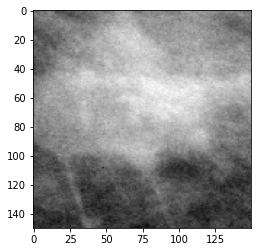
\includegraphics[scale=0.6]{./img/dataOriginal.png}
    \end{minipage}
\end{center}


\begin{minipage}{0.01\textwidth}
        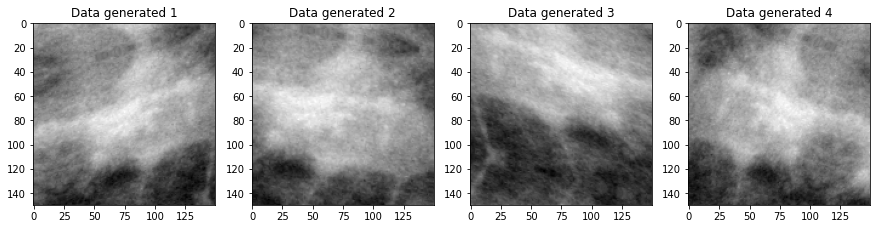
\includegraphics[scale=0.38]{./img/dataGen.png}
    \end{minipage}


%---------------- model1, augmented data ------------------------
\subsubsection{Model 1, trained on augmented data}

\begin{verbatim}

              precision    recall  f1-score   support

           0       0.77      0.74      0.75       219
           1       0.54      0.59      0.57       117

    accuracy                           0.68       336
   macro avg       0.66      0.66      0.66       336
weighted avg       0.69      0.68      0.69       336

0s 9ms/step - loss: 0.6145 - accuracy: 0.6845

\end{verbatim}


\begin{figure}[h]
    \centering
    \begin{minipage}{0.45\textwidth}
        \centering
        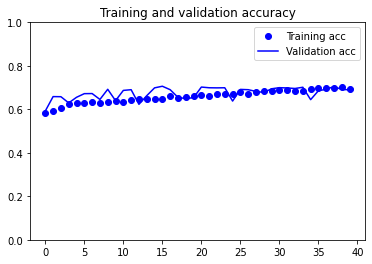
\includegraphics[scale=0.46]{./img/scratchVal2_2.png}
    \end{minipage}\hfill
    \begin{minipage}{0.45\textwidth}
        \centering
        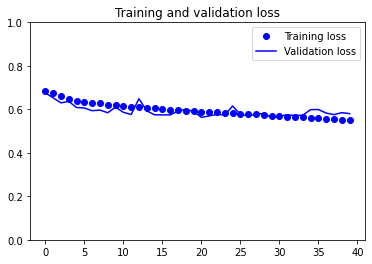
\includegraphics[scale=0.46]{./img/scratchLoss2_2.png}
    \end{minipage}
\end{figure}

\begin{center}
\begin{minipage}{0.45\textwidth}
        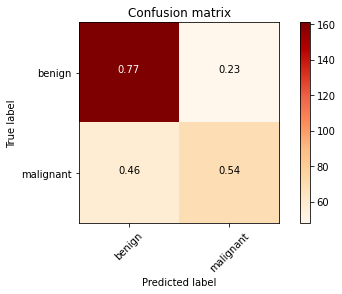
\includegraphics[scale=0.6]{./img/cmScratch2_2.png}
    \end{minipage}
\end{center}
We improved our classifier, obtaining an increasing about 4\% on the accuracy value and a decreasing on the loss value of 3\%.




%------------------ model2, augmented data ---------------------
\subsubsection{Model 2, trained on augmented data}
Comparing the results of the previous model trained on augmeneted data and orginal data, we decided to use the data augmentation techique to train all the following models of this task.

\begin{itemize}
\item Optimizer: RMSProp, learning rate = 1e-4
\item Early stopping condition: monitoring loss on validation set, patience = 10
\item Dense hidden layers: 2
\item Activation function: sigmoid
\end{itemize}
\begin{verbatim}

              precision    recall  f1-score   support

           0       0.79      0.58      0.67       219
           1       0.47      0.72      0.57       117

    accuracy                           0.62       336
   macro avg       0.63      0.65      0.62       336
weighted avg       0.68      0.62      0.63       336

0s 21ms/step - loss: 0.6429 - accuracy: 0.6250

\end{verbatim}


\begin{figure}[h]
    \centering
    \begin{minipage}{0.45\textwidth}
        \centering
        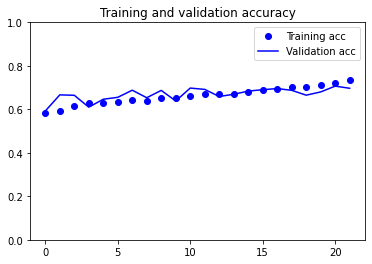
\includegraphics[scale=0.46]{./img/scratchVal3_2.png}
    \end{minipage}\hfill
    \begin{minipage}{0.45\textwidth}
        \centering
        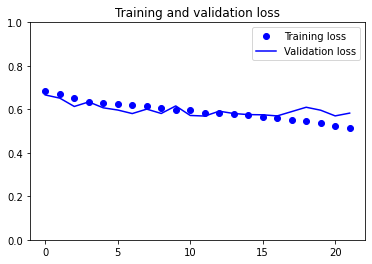
\includegraphics[scale=0.46]{./img/scratchLoss3_2.png}
    \end{minipage}
\end{figure}

\begin{center}
\begin{minipage}{0.45\textwidth}
        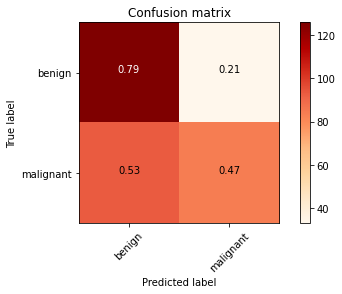
\includegraphics[scale=0.6]{./img/cmScratch3_2.png}
    \end{minipage}
\end{center}
Complicating the architecture of the network, adding more layers, we didn't improve the results.


%------------------ model3, augmented data ---------------------
\subsubsection{Model 3, trained on augmented data}

\begin{itemize}
\item Optimizer: Adam, learning rate = 0.001 (default)
\item Early stopping condition: monitoring loss on validation set, patience = 10
\item Dense hidden layers: 2
\item Dropout layer between the 2 dense layers: rate = 0.2
\item Activation function: sigmoid
\end{itemize}
\begin{verbatim}

              precision    recall  f1-score   support

           0       0.71      0.81      0.76       219
           1       0.52      0.38      0.44       117

    accuracy                           0.66       336
   macro avg       0.61      0.59      0.60       336
weighted avg       0.64      0.66      0.65       336

0s 21ms/step - loss: 0.6186 - accuracy: 0.6607

\end{verbatim}


\begin{figure}[h]
    \centering
    \begin{minipage}{0.45\textwidth}
        \centering
        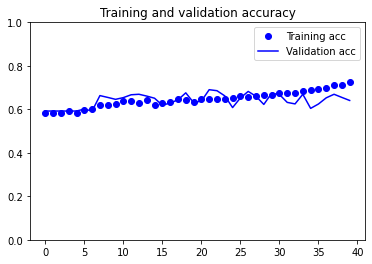
\includegraphics[scale=0.46]{./img/scratchVal4_2.png}
    \end{minipage}\hfill
    \begin{minipage}{0.45\textwidth}
        \centering
        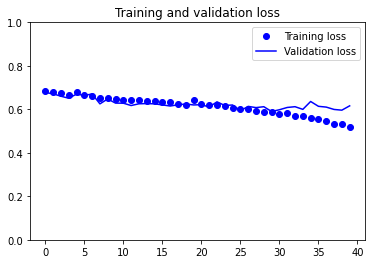
\includegraphics[scale=0.46]{./img/scratchLoss4_2.png}
    \end{minipage}
\end{figure}

\begin{center}
\begin{minipage}{0.45\textwidth}
        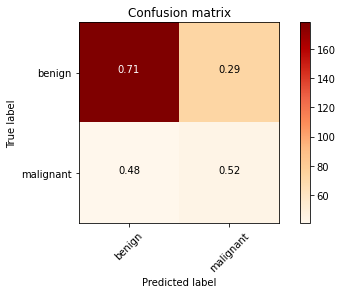
\includegraphics[scale=0.6]{./img/cmScratch4_2.png}
    \end{minipage}
\end{center}

% ------
\subsection{Conclusion task 2.2}
We ploted the roc curve related to each of the built models and we compared them.
\begin{center}
\begin{minipage}{0.45\textwidth}
        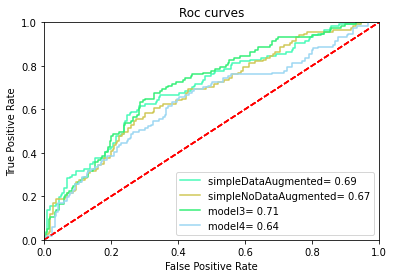
\includegraphics[scale=0.6]{./img/rocScratch2.png}
    \end{minipage}
\end{center}
We select the first model as best classifier, despite its area under the roc is less than the third one, because it classifies better the class Malignant.\\
The area under the roc equal to 0.71 related to the third classifier is given basically by the high accuracy in the correct classification of class Benign.










\clearpage
% --------------------------------------- TASK 3 -------------------------------------------------------
\section{Task 3}
Task 3 consists in development different models exploiting a pretrained convolotional neural networks able to compute the following classification:
\begin{itemize}
\item Mass - Calcification
\item Benign - Malignant
\end{itemize}
Reading different papers and guides, we identified the most common used pretrained networks for images classification:
\begin{itemize}
\item ResNet
\item GoogleNet
\item VGG
\end{itemize}
For each of these networks, we used different versions and variants, for ResNet we tried ResNet50 and ResNet152; for GoogleNet we used the most recent variant InceptionV3 (while GoogleNet is called InceptionV1); for VGG we use VGG16 and VGG19.\\
Considering we used some pretrained networks, we followed the good practise and we decreased the learning rate respect to the task 2.1.\\
Another consideration to make is to note that all each pretrained neural network that we imported on the project, has been trained on a dataset composed by colored RBG images. Instead our dataset is composed by grayscale images; we found a solution which consists in replicating three times the image over the tree channels (Red - Green - Blue).



% --------------------------------------- TASK 3.1 -------------------------------------------------------
\subsection{Task 3.1, Mass - Calcification}
We tried to solve this task following two approaches:
\begin{itemize}
\item Features extraction
\item Fine tuning
\end{itemize}
We trained all the models of this task on an augmented dataset, generated using the same value of the DataImageGenerator of the task 2.2.

%-------------------- vgg16 feature extraction ----------------------
\subsubsection{Model 1, VGG16 features extraction}
The first pretrained network used is VGG16. We cobined this pretrained network (freezing all layers) to a fully connected classifier, composed by two hidden layers.\\

\begin{itemize}
\item Optimizer: RMSProp, learning rate = 2e-6
\item Early stopping condition: monitoring loss on validation set, patience = 10
\item Dense hidden layers: 2
\item Activation function: sigmoid
\end{itemize}

\begin{verbatim}


              precision    recall  f1-score   support

           0       0.81      0.88      0.85       179
           1       0.85      0.77      0.81       157

    accuracy                           0.83       336
   macro avg       0.83      0.83      0.83       336
weighted avg       0.83      0.83      0.83       336

1s 62ms/step - loss: 0.3738 - accuracy: 0.8304

\end{verbatim}


\begin{figure}[h]
    \centering
    \begin{minipage}{0.45\textwidth}
        \centering
        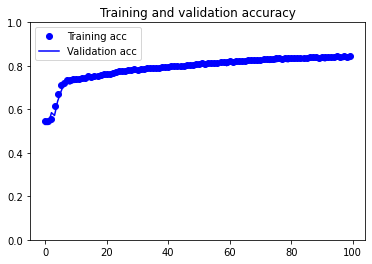
\includegraphics[scale=0.46]{./img/preTrainVal3_fe.png}
    \end{minipage}\hfill
    \begin{minipage}{0.45\textwidth}
        \centering
        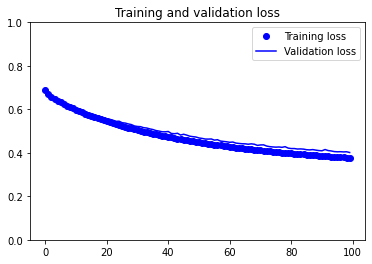
\includegraphics[scale=0.46]{./img/preTrainLoss3_fe.png}
    \end{minipage}
\end{figure}

\begin{center}
\begin{minipage}{0.45\textwidth}
        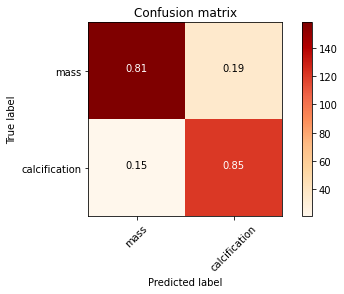
\includegraphics[scale=0.6]{./img/cmPreTrain3_fe.png}
    \end{minipage}
\end{center}



%-------------------- vgg16 fine tuning ----------------------
\subsubsection{Model 1, VGG16 fine tuning}
We freezed all the layers of the original model, except the first layer of the last block: \textit{block5\_conv1}.

\begin{itemize}
\item Optimizer: RMSProp, learning rate = 2e-6
\item Early stopping condition: monitoring loss on validation set, patience = 10
\item Dense hidden layers: 2
\item Activation function: sigmoid
\end{itemize}

\begin{verbatim}


              precision    recall  f1-score   support

           0       0.87      0.91      0.89       179
           1       0.89      0.85      0.87       157

    accuracy                           0.88       336
   macro avg       0.88      0.88      0.88       336
weighted avg       0.88      0.88      0.88       336

1s 62ms/step - loss: 0.2983 - accuracy: 0.8810

\end{verbatim}

\begin{figure}[h]
    \centering
    \begin{minipage}{0.45\textwidth}
        \centering
        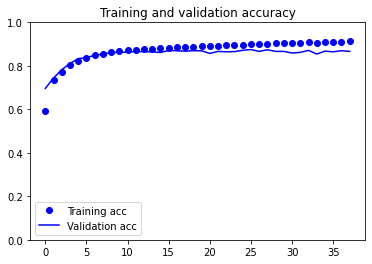
\includegraphics[scale=0.46]{./img/preTrainVal3_ft.png}
    \end{minipage}\hfill
    \begin{minipage}{0.45\textwidth}
        \centering
        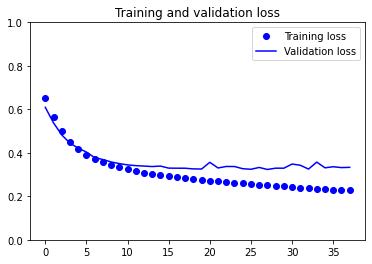
\includegraphics[scale=0.46]{./img/preTrainLoss3_ft.png}
    \end{minipage}
\end{figure}

\begin{center}
\begin{minipage}{0.45\textwidth}
        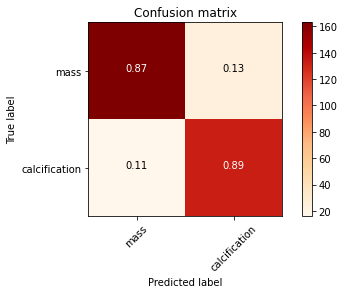
\includegraphics[scale=0.6]{./img/cmPreTrain3_ft.png}
    \end{minipage}
\end{center}

\subsubsection{VGG16: features extraction VS fine tuning}
Applying the fine tuning technique to VGG16, we obtained about 4\% more on the area under the curve than the features extraction technique.
\begin{center}
\begin{minipage}{0.45\textwidth}
        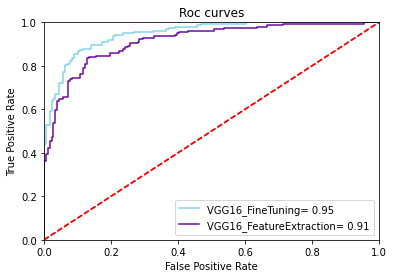
\includegraphics[scale=0.6]{./img/rocVGG16.png}
    \end{minipage}
\end{center}



%-------------------- vgg19 feature extraction ----------------------
\subsubsection{Model 2, VGG19 features extraction}
The second pretrained network used, as alternative to VGG16, is VGG19. Also in this case we cobined this pretrained network to a fully connected classifier, composed by two hidden layers, than we freezed all the layers of the original model, in order to implement the features extraction technique.

\begin{itemize}
\item Optimizer: RMSProp, learning rate = 2e-6
\item Early stopping condition: monitoring loss on validation set, patience = 10
\item Dense hidden layers: 2
\item Activation function: sigmoid
\end{itemize}

\begin{verbatim}


              precision    recall  f1-score   support

           0       0.85      0.81      0.83       179
           1       0.79      0.83      0.81       157

    accuracy                           0.82       336
   macro avg       0.82      0.82      0.82       336
weighted avg       0.82      0.82      0.82       336

1s 74ms/step - loss: 0.4191 - accuracy: 0.8214

\end{verbatim}


\begin{figure}[h]
    \centering
    \begin{minipage}{0.45\textwidth}
        \centering
        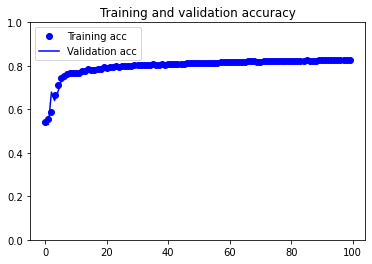
\includegraphics[scale=0.46]{./img/preTrainValVGG19_fe.png}
    \end{minipage}\hfill
    \begin{minipage}{0.45\textwidth}
        \centering
        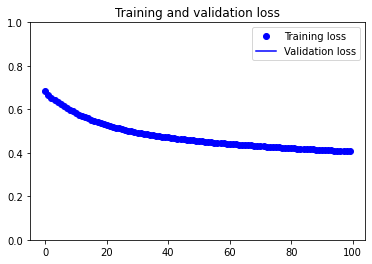
\includegraphics[scale=0.46]{./img/preTrainLossVGG19_fe.png}
    \end{minipage}
\end{figure}

\begin{center}
\begin{minipage}{0.45\textwidth}
        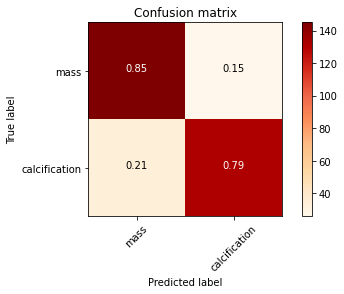
\includegraphics[scale=0.6]{./img/cmPreTrainVGG19_fe.png}
    \end{minipage}
\end{center}



%-------------------- vgg19 fine tuning ----------------------
\subsubsection{Model 2, VGG19 fine tuning}
We applied the fine tuning also to this pretrained neural network: we freezed all the layers of the original model, except the first layer of the last block: \textit{block5\_conv1}.

\begin{itemize}
\item Optimizer: RMSProp, learning rate = 2e-6
\item Early stopping condition: monitoring loss on validation set, patience = 10
\item Dense hidden layers: 2
\item Activation function: sigmoid
\end{itemize}

\begin{verbatim}


              precision    recall  f1-score   support

           0       0.88      0.87      0.87       179
           1       0.85      0.86      0.85       157

    accuracy                           0.86       336
   macro avg       0.86      0.86      0.86       336
weighted avg       0.86      0.86      0.86       336

1s 75ms/step - loss: 0.3346 - accuracy: 0.8631

\end{verbatim}

\begin{figure}[h]
    \centering
    \begin{minipage}{0.45\textwidth}
        \centering
        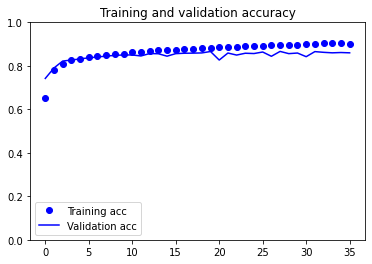
\includegraphics[scale=0.46]{./img/preTrainValVGG19_ft.png}
    \end{minipage}\hfill
    \begin{minipage}{0.45\textwidth}
        \centering
        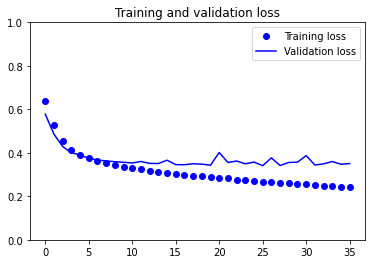
\includegraphics[scale=0.46]{./img/preTrainLossVGG19_ft.png}
    \end{minipage}
\end{figure}

\begin{center}
\begin{minipage}{0.45\textwidth}
        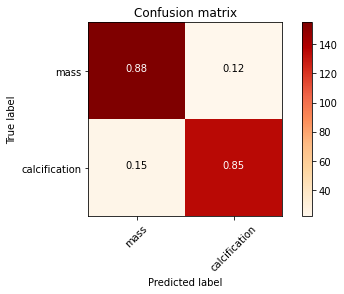
\includegraphics[scale=0.6]{./img/cmPreTrainVGG19_ft.png}
    \end{minipage}
\end{center}

\subsubsection{VGG19: features extraction VS fine tuning}
Applying the fine tuning technique to VGG19, we obtained about 4\% more on the area under the curve than the features extraction technique.
\begin{center}
\begin{minipage}{0.45\textwidth}
        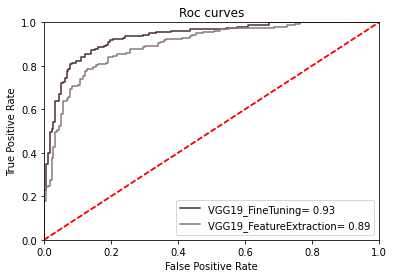
\includegraphics[scale=0.6]{./img/rocVGG19.png}
    \end{minipage}
\end{center}






%-------------------- ResNet50 feature extraction ----------------------
\subsubsection{Model 3, ResNet50 features extraction}
The third pretrained network used is ResNet50. In this case we cobined this pretrained network to a fully connected classifier, composed by a single hidden layers, than we freezed all the layers of the original model, in order to implement the features extraction technique.

\begin{itemize}
\item Optimizer: RMSProp, learning rate = 2e-6
\item Early stopping condition: monitoring loss on validation set, patience = 10
\item Dense hidden layers: 1
\item Activation function: sigmoid
\end{itemize}

\begin{verbatim}


              precision    recall  f1-score   support

           0       0.80      0.56      0.66       179
           1       0.63      0.84      0.72       157

    accuracy                           0.69       336
   macro avg       0.72      0.70      0.69       336
weighted avg       0.72      0.69      0.69       336

1s 50ms/step - loss: 0.6555 - accuracy: 0.6935

\end{verbatim}


\begin{figure}[h]
    \centering
    \begin{minipage}{0.45\textwidth}
        \centering
        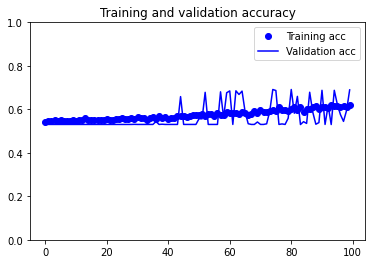
\includegraphics[scale=0.46]{./img/preTrainValResNet50_fe.png}
    \end{minipage}\hfill
    \begin{minipage}{0.45\textwidth}
        \centering
        \includegraphics[scale=0.46]{./img/preTrainLossResNet50_fe.png}
    \end{minipage}
\end{figure}

\begin{center}
\begin{minipage}{0.45\textwidth}
        \includegraphics[scale=0.6]{./img/cmPreTrainResNet50_fe.png}
    \end{minipage}
\end{center}



%-------------------- ResNet50 fine tuning ----------------------
\subsubsection{Model 3, ResNet50 fine tuning}
We applied the fine tuning also to this pretrained neural network: we freezed all the layers of the original model, except the first layer of the last block: \textit{block5\_conv1}.

\begin{itemize}
\item Optimizer: RMSProp, learning rate = 2e-6
\item Early stopping condition: monitoring loss on validation set, patience = 10
\item Dense hidden layers: 1
\item Activation function: sigmoid
\end{itemize}

\begin{verbatim}


              precision    recall  f1-score   support

           0       0.80      0.93      0.86       179
           1       0.91      0.73      0.81       157

    accuracy                           0.84       336
   macro avg       0.85      0.83      0.84       336
weighted avg       0.85      0.84      0.84       336

1s 51ms/step - loss: 0.3897 - accuracy: 0.8393

\end{verbatim}

\begin{figure}[h]
    \centering
    \begin{minipage}{0.45\textwidth}
        \centering
        \includegraphics[scale=0.46]{./img/preTrainValResNet50_ft.png}
    \end{minipage}\hfill
    \begin{minipage}{0.45\textwidth}
        \centering
        \includegraphics[scale=0.46]{./img/preTrainLossResNet50_ft.png}
    \end{minipage}
\end{figure}

\begin{center}
\begin{minipage}{0.45\textwidth}
        \includegraphics[scale=0.6]{./img/cmPreTrainResNet50_ft.png}
    \end{minipage}
\end{center}

\subsubsection{ResNet50: features extraction VS fine tuning}
Applying the fine tuning technique to ResNet50, we obtained about 14\% more on the area under the curve than the features extraction technique.
\begin{center}
\begin{minipage}{0.45\textwidth}
        \includegraphics[scale=0.6]{./img/rocResNet50.png}
    \end{minipage}
\end{center}






%-------------------- InceptionV3 feature extraction ----------------------
\subsubsection{Model 4, InceptionV3 features extraction}
The fourth and last pretrained network used is InceptionV3. Also this case we cobined this pretrained network to a fully connected classifier, composed by a single hidden layers, as in the previous case. Than we freezed all the layers of the original model, in order to implement the features extraction technique.

\begin{itemize}
\item Optimizer: RMSProp, learning rate = 2e-6
\item Early stopping condition: monitoring loss on validation set, patience = 10
\item Dense hidden layers: 1
\item Activation function: sigmoid
\end{itemize}

\begin{verbatim}


              precision    recall  f1-score   support

           0       0.86      0.89      0.88       179
           1       0.87      0.84      0.86       157

    accuracy                           0.87       336
   macro avg       0.87      0.87      0.87       336
weighted avg       0.87      0.87      0.87       336

0s 31ms/step - loss: 0.3268 - accuracy: 0.8690

\end{verbatim}


\begin{figure}[h]
    \centering
    \begin{minipage}{0.45\textwidth}
        \centering
        \includegraphics[scale=0.46]{./img/preTrainValInception_fe.png}
    \end{minipage}\hfill
    \begin{minipage}{0.45\textwidth}
        \centering
        \includegraphics[scale=0.46]{./img/preTrainLossInception_fe.png}
    \end{minipage}
\end{figure}

\begin{center}
\begin{minipage}{0.45\textwidth}
        \includegraphics[scale=0.6]{./img/cmPreTrainInception_fe.png}
    \end{minipage}
\end{center}



%-------------------- InceptionV3 fine tuning ----------------------
\subsubsection{Model 4, InceptionV3 fine tuning}
We applied the fine tuning also to this pretrained neural network: we freezed all the layers of the original model, except the first layer of the last block: \textit{conv2d\_93}.

\begin{itemize}
\item Optimizer: RMSProp, learning rate = 2e-6
\item Early stopping condition: monitoring loss on validation set, patience = 10
\item Dense hidden layers: 1
\item Activation function: sigmoid
\end{itemize}

\begin{verbatim}


              precision    recall  f1-score   support

           0       0.86      0.90      0.88       179
           1       0.88      0.83      0.85       157

    accuracy                           0.87       336
   macro avg       0.87      0.86      0.86       336
weighted avg       0.87      0.87      0.87       336

0s 31ms/step - loss: 0.3288 - accuracy: 0.8661

\end{verbatim}

\begin{figure}[h]
    \centering
    \begin{minipage}{0.45\textwidth}
        \centering
        \includegraphics[scale=0.46]{./img/preTrainValInception_ft.png}
    \end{minipage}\hfill
    \begin{minipage}{0.45\textwidth}
        \centering
        \includegraphics[scale=0.46]{./img/preTrainLossInception_ft.png}
    \end{minipage}
\end{figure}

\begin{center}
\begin{minipage}{0.45\textwidth}
        \includegraphics[scale=0.6]{./img/cmPreTrainInception_ft.png}
    \end{minipage}
\end{center}

\subsubsection{InceptionV3: features extraction VS fine tuning}
Applying the features extraction and fine tuning techniques to InceptionV3 neural network, we obtained the same results in terms of accurancy and loss.
\begin{center}
\begin{minipage}{0.45\textwidth}
        \includegraphics[scale=0.6]{./img/rocInception.png}
    \end{minipage}
\end{center}

% ------
\subsection{Comparison between the models of the task 3.1}
We ploted the roc curve related to each of the models built using the fine tuning technique, because it gives better models than features extraction (except for InceptionV3) and we compared them.
\begin{center}
\begin{minipage}{0.45\textwidth}
        \includegraphics[scale=0.6]{./img/rocPretrain1.png}
    \end{minipage}
\end{center}
We saved the models based on VGG16, VGG19 and InceptionV3, in order to use them in the task 5.










\clearpage
% --------------------------------------- TASK 3.2 -------------------------------------------------------
\subsection{Task 3.2, Benign - Malignant}
Also in this case we tried to solve this classification problem with both features extraction and fine tuning, but unlike the previous task, in some cases we obtained better results using features extraction technique, others using fine tuning.\\
Moreover we imported the same pretrained networks, trained on imagenet dataset.\\
We combined two approaches, in order to rebalance the two classes.
\begin{itemize}
\item Data augmentation, using \textit{ImageDataGenerator}, basically to increase the dimension of the dataset, in order to use the fine tuning technique.
\item Assign different weights to the two classes, basically to give more importance to the malignant one, that is more critical to detect.
\end{itemize}
We tried some formulas, in order to try different values of weights :

\begin{verbatim}
weightsBenign = malignantNum / (malignantNum + benignNum)
weightsMalignant = benignNum / (malignantNum + benignNum) 
weights = { 0: weightsBenign * 2,  1: (weightsMalignant + 0.3) * 2}

0.828101644245142
1.7718983557548578


weightsBenign = malignantNum / (malignantNum + benignNum)
weightsMalignant = benignNum / (malignantNum + benignNum) 
weights = { 0: weightsBenign - .05, 1: weightsMalignant + .05}

0.364050822122571
0.635949177877429


weightsBenign = malignantNum / min(malignantNum, benignNum)
weightsMalignant = benignNum / min(malignantNum, benignNum) 
weights = { 0: weightsBenign, 1: weightsMalignant}

1.0
1.4151624548736461

\end{verbatim}
After some experiments we decided to use the third couple of weights:\\ \textit{weights = \{ 0: 1.0 ,   1: 1.415... \}}

%-------------------- vgg16 fine tuning ----------------------
\subsubsection{Model 1, VGG16 fine tuning}
We freezed all the layers of the original model, except the first layer of the last block: \textit{block5\_conv1}.

\begin{itemize}
\item Optimizer: RMSProp, learning rate = 2e-6
\item Early stopping condition: monitoring loss on validation set, patience = 10
\item Dense hidden layers: 2
\item Dropout layers between the dense hidden one: rate = 0.5
\item Activation function: sigmoid
\end{itemize}

\begin{verbatim}


              precision    recall  f1-score   support

           0       0.77      0.72      0.74       219
           1       0.53      0.59      0.56       117

    accuracy                           0.68       336
   macro avg       0.65      0.66      0.65       336
weighted avg       0.68      0.68      0.68       336

1s 63ms/step - loss: 0.6062 - accuracy: 0.6756

\end{verbatim}

\begin{figure}[h]
    \centering
    \begin{minipage}{0.45\textwidth}
        \centering
        \includegraphics[scale=0.46]{./img/preTrainValVGG16_ft_3_2.png}
    \end{minipage}\hfill
    \begin{minipage}{0.45\textwidth}
        \centering
        \includegraphics[scale=0.46]{./img/preTrainLossVGG16_ft_3_2.png}
    \end{minipage}
\end{figure}


\begin{center}
\begin{minipage}{0.45\textwidth}
        \includegraphics[scale=0.6]{./img/cmPreTrainVGG16_ft_3_2.png}
    \end{minipage}
\end{center}




%-------------------- vgg19 fine tuning ----------------------
\subsubsection{Model 2, VGG19 fine tuning}
We applied the fine tuning also to this pretrained neural network: we freezed all the layers of the original model, except the first layer of the last block: \textit{block5\_conv1}.

\begin{itemize}
\item Optimizer: RMSProp, learning rate = 2e-6
\item Early stopping condition: monitoring loss on validation set, patience = 10
\item Dense hidden layers: 2
\item Dropout layers between the dense hidden one: rate = 0.5
\item Activation function: sigmoid
\end{itemize}

\begin{verbatim}


              precision    recall  f1-score   support

           0       0.74      0.75      0.75       219
           1       0.52      0.51      0.52       117

    accuracy                           0.67       336
   macro avg       0.63      0.63      0.63       336
weighted avg       0.67      0.67      0.67       336

1s 78ms/step - loss: 0.6144 - accuracy: 0.6667

\end{verbatim}

\begin{figure}[h]
    \centering
    \begin{minipage}{0.45\textwidth}
        \centering
        \includegraphics[scale=0.46]{./img/preTrainValVGG19_ft_3_2.png}
    \end{minipage}\hfill
    \begin{minipage}{0.45\textwidth}
        \centering
        \includegraphics[scale=0.46]{./img/preTrainLossVGG19_ft_3_2.png}
    \end{minipage}
\end{figure}

\begin{center}
\begin{minipage}{0.45\textwidth}
        \includegraphics[scale=0.6]{./img/cmPreTrainVGG19_ft_3_2.png}
    \end{minipage}
\end{center}



%-------------------- ResNet50 fine tuning ----------------------
\subsubsection{Model 3, ResNet50 features extraction}
We applied the fine tuning also to this pretrained neural network: we freezed all the layers of the original model.

\begin{itemize}
\item Optimizer: RMSProp, learning rate = 2e-6
\item Early stopping condition: monitoring loss on validation set, patience = 10
\item Dense hidden layers: 1
\item Dropout layers between the dense hidden layer and the output one: rate = 0.5
\item Activation function: sigmoid
\end{itemize}

\begin{verbatim}


              precision    recall  f1-score   support

           0       0.65      1.00      0.79       219
           1       0.67      0.02      0.03       117

    accuracy                           0.65       336
   macro avg       0.66      0.51      0.41       336
weighted avg       0.66      0.65      0.53       336

1s 50ms/step - loss: 0.6869 - accuracy: 0.6548

\end{verbatim}

\begin{figure}[h]
    \centering
    \begin{minipage}{0.45\textwidth}
        \centering
        \includegraphics[scale=0.46]{./img/preTrainValResNet_ft_3_2.png}
    \end{minipage}\hfill
    \begin{minipage}{0.45\textwidth}
        \centering
        \includegraphics[scale=0.46]{./img/preTrainLossResNet_ft_3_2.png}
    \end{minipage}
\end{figure}

\begin{center}
\begin{minipage}{0.45\textwidth}
        \includegraphics[scale=2.6]{./img/cmPreTrainResNet_ft_3_2.png}
    \end{minipage}
\end{center}



%-------------------- InceptionV3 fine tuning ----------------------
\subsubsection{Model 4, InceptionV3 features extraction}
We applied the fine tuning also to this pretrained neural network: we freezed all the layers of the original model.

\begin{itemize}
\item Optimizer: RMSProp, learning rate = 2e-6
\item Early stopping condition: monitoring loss on validation set, patience = 10
\item Dense hidden layers: 1
\item Dropout layers between the dense hidden layer and the output one: rate = 0.5
\item Activation function: sigmoid
\end{itemize}

\begin{verbatim}


              precision    recall  f1-score   support

           0       0.83      0.68      0.75       219
           1       0.55      0.74      0.64       117

    accuracy                           0.70       336
   macro avg       0.69      0.71      0.69       336
weighted avg       0.74      0.70      0.71       336

0s 30ms/step - loss: 0.5773 - accuracy: 0.7024

\end{verbatim}

\begin{figure}[h]
    \centering
    \begin{minipage}{0.45\textwidth}
        \centering
        \includegraphics[scale=0.46]{./img/preTrainValInception_ft_3_2.png}
    \end{minipage}\hfill
    \begin{minipage}{0.45\textwidth}
        \centering
        \includegraphics[scale=0.46]{./img/preTrainLossInception_ft_3_2.png}
    \end{minipage}
\end{figure}

\begin{center}
\begin{minipage}{0.45\textwidth}
        \includegraphics[scale=0.6]{./img/cmPreTrainInception_ft_3_2.png}
    \end{minipage}
\end{center}

% ------
\subsection{Comparison between the models of the task 3.2}
We ploted the roc curve related to each of the models shown in the previous paragraphs and we compared them.
\begin{center}
\begin{minipage}{0.45\textwidth}
        \includegraphics[scale=0.6]{./img/rocPretrain3_2.png}
    \end{minipage}
\end{center}
We saved the top 3 models: those based on VGG16 (fine tuning), VGG19 (fine tuning), and InceptionV3 (features extractions), in order to use them in the task 5.




\clearpage
% --------------------------------------- TASK 4 -------------------------------------------------------
\section{Task 4}
We tried to increase the results of task 3.2 exploiting the baseline patches, using different approaches:
\begin{itemize}
\item \textbf{Siamese network}
\item \textbf{Hilghlight the abnormality portion} using the baseline patches and a pretrained network
\end{itemize}

\subsection{Siamese architecture}
We implemented a siamese neural network, as shown on the following picture; where the two sisters networks are VGG16 pretrained on the dataset imagenet.\\
We tried to impelment the merge layer following two different approaches:
\begin{itemize}
\item Concatenate the output of the siters networks
\item Compute the difference element by element between the output of the siters networks
\end{itemize}
Finally there is the classifier composed by a single dense hidden layer.\\

\subsubsection{Siamese, implementing the concatenation}
\begin{minipage}{0.45\textwidth}
        \includegraphics[scale=0.32]{./img/siamese_concat.png}
\end{minipage}

\begin{verbatim}
              precision    recall  f1-score   support
           0       0.78      0.73      0.75       219
           1       0.55      0.62      0.58       117

    accuracy                           0.69       336
   macro avg       0.67      0.67      0.67       336
weighted avg       0.70      0.69      0.69       336

1s 133ms/step - loss: 0.5700 - accuracy: 0.6905
\end{verbatim}

\begin{figure}[h]
    \centering
    \begin{minipage}{0.45\textwidth}
        \centering
        \includegraphics[scale=0.4]{./img/siamese_concat_accuracy.png}
    \end{minipage}\hfill
    \begin{minipage}{0.45\textwidth}
        \centering
        \includegraphics[scale=0.4]{./img/siamese_concat_loss.png}
    \end{minipage}
\end{figure}



\subsubsection{Siamese, implementing the difference}
\begin{minipage}{0.45\textwidth}
        \includegraphics[scale=0.32]{./img/siamese_diff.png}
\end{minipage}

\begin{verbatim}
precision    recall  f1-score   support
           0       0.73      0.70      0.71       219
           1       0.48      0.52      0.50       117

    accuracy                           0.64       336
   macro avg       0.61      0.61      0.61       336
weighted avg       0.64      0.64      0.64       336

1s 133ms/step - loss: 0.6231 - accuracy: 0.6369
\end{verbatim}



\begin{figure}[h]
    \centering
    \begin{minipage}{0.45\textwidth}
        \centering
        \includegraphics[scale=0.4]{./img/siamese_concat_accuracy.png}
    \end{minipage}\hfill
    \begin{minipage}{0.45\textwidth}
        \centering
        \includegraphics[scale=0.4]{./img/siamese_concat_loss.png}
    \end{minipage}
\end{figure}


\iffalse
\begin{figure}[h]
    \centering
    \begin{minipage}{0.45\textwidth}
        \centering
        \includegraphics[scale=0.46]{./img/siamese_diff_acc.png}
    \end{minipage}\hfill
    \begin{minipage}{0.45\textwidth}
        \centering
        \includegraphics[scale=0.46]{./img/siamese_diff_loss.png}
    \end{minipage}
\end{figure}
\fi


\subsubsection{Conclusion of Siamese network}
After implementing this architecture, we compare the results obtained with those obtained on task 3.2 and we increased the accurancy about 2 - 3\% respect to VGG16, VGG19 and ResNet50 and the same results respect to the InceptionV3.


\subsection{Pretrained network}
The other approach we followed to use the baseline patches to improve the accuracy of our models, trying to remove the healthy tissue part from the abnormality images.\\
The intuition of this technique is the following: we aspected an uniform distribution of color in the baseline images and some small portions of healthy tissue in the abnormality ones, so we would highlight the abnormality, computing the difference berween the two images.
\begin{figure}[H]
    \centering
    \begin{minipage}{0.45\textwidth}
        \centering
        \includegraphics[scale=0.56]{./img/abnormality.png}
	\caption{Abnormality}
    \end{minipage}\hfill
    \begin{minipage}{0.45\textwidth}
        \centering
        \includegraphics[scale=0.56]{./img/baseline.png}
\caption{Baseline patch}
    \end{minipage}
\end{figure}\vspace{1mm}By observing the baseline image, we can say that the color is not plane as we expected, so we compute the mean value of the matrix, in order to force color uniformity. \\

\begin{figure}[H]
    \centering
    \begin{minipage}{0.45\textwidth}
        \centering
        \includegraphics[scale=0.56]{./img/baselineAvg.png}
	\caption{Mean value of the healthy image}
    \end{minipage}\hfill
    \begin{minipage}{0.45\textwidth}
        \centering
        \includegraphics[scale=0.56]{./img/diffBaseline.png}
\caption{Difference between abnormality and the mean of baseline}
    \end{minipage}
\end{figure}
After implementing this intuition we obtained the same value of the accuracy and an increase of the loss. Trying to emphasize the abnormality, we actually remove part of infomation.



\clearpage
% --------------------------------------- TASK 5 -------------------------------------------------------
\section{Task 5, Ensemble}
In this task we combined different models that we saved for each classification problem, except for task 2.2, where we saved a single model, implementing the following approaches:
\begin{itemize}
\item Average voting
\item Majoring voting
\end{itemize}

\subsection{Enseble, task 2.1}
\subsubsection{Average Voting}

\begin{verbatim}

              precision    recall  f1-score   support

           0       0.83      0.87      0.85       179
           1       0.84      0.80      0.82       157

    accuracy                           0.84       336
   macro avg       0.84      0.83      0.84       336
weighted avg       0.84      0.84      0.84       336

\end{verbatim}

\begin{center}
\begin{minipage}{0.45\textwidth}
        \includegraphics[scale=0.6]{./img/cmEnsAvg2_1.png}
    \end{minipage}
\end{center}

\subsubsection{Majority Voting}
\begin{verbatim}

              precision    recall  f1-score   support

           0       0.84      0.86      0.85       179
           1       0.84      0.82      0.83       157

    accuracy                           0.84       336
   macro avg       0.84      0.84      0.84       336
weighted avg       0.84      0.84      0.84       336

\end{verbatim}

\begin{center}
\begin{minipage}{0.45\textwidth}
        \includegraphics[scale=0.6]{./img/cmEnsMaj2_1.png}
    \end{minipage}
\end{center}



\subsection{Enseble, task 3.1}
\subsubsection{Average Voting}

\begin{verbatim}

              precision    recall  f1-score   support

           0       0.91      0.91      0.91       179
           1       0.89      0.89      0.89       157

    accuracy                           0.90       336
   macro avg       0.90      0.90      0.90       336
weighted avg       0.90      0.90      0.90       336

\end{verbatim}

\begin{center}
\begin{minipage}{0.45\textwidth}
        \includegraphics[scale=0.6]{./img/cmEnsAvg3_1.png}
    \end{minipage}
\end{center}

\subsubsection{Majority Voting}
\begin{verbatim}

              precision    recall  f1-score   support

           0       0.90      0.89      0.89       179
           1       0.87      0.89      0.88       157

    accuracy                           0.89       336
   macro avg       0.89      0.89      0.89       336
weighted avg       0.89      0.89      0.89       336

\end{verbatim}

\begin{center}
\begin{minipage}{0.45\textwidth}
        \includegraphics[scale=0.6]{./img/cmEnsMaj3_1.png}
    \end{minipage}
\end{center}



\subsection{Enseble, task 3.2}
\subsubsection{Average Voting}

\begin{verbatim}

              precision    recall  f1-score   support

           0       0.79      0.74      0.77       219
           1       0.57      0.62      0.59       117

    accuracy                           0.70       336
   macro avg       0.68      0.68      0.68       336
weighted avg       0.71      0.70      0.71       336

\end{verbatim}

\begin{center}
\begin{minipage}{0.45\textwidth}
        \includegraphics[scale=0.6]{./img/cmEnsAvg3_2.png}
    \end{minipage}
\end{center}

\subsubsection{Majority Voting}
\begin{verbatim}

              precision    recall  f1-score   support

           0       0.78      0.75      0.77       219
           1       0.57      0.62      0.59       117

    accuracy                           0.70       336
   macro avg       0.68      0.68      0.68       336
weighted avg       0.71      0.70      0.71       336

\end{verbatim}

\begin{center}
\begin{minipage}{0.45\textwidth}
        \includegraphics[scale=0.6]{./img/cmEnsMaj3_2.png}
    \end{minipage}
\end{center}



\subsection{Conclusion Ensembling}
Looking the results obtained in this task, we can observe in same cases a small increase on the accuracy respect of some single models, in others the performaces remains unchanged.\\
Generally the average voting gives better results than majority voting, about 1\%.





\end{document}